\chapter{Background}
\label{ch:background}
This chapter explains the methods and concepts. These are separated in 3 parts: one for basic knowledge, one for the evaluation methods used, and one for the used models. 

\section{Basic Knowledge}
Important knowledge for understanding the contents of the thesis: this includes how an encoder-decoder model can generate an output sequence; what machine translation, automatic Speech recognition, and dropout are; and a section about the Models used, the different basic model architectures, and an explanation of the model architectures of the specific models used in the experiments.

\subsection{Sequence Generation}\label{sect: sequence generation}
An encoder-decoder model generates a sequence $y=(y_1\dots y_m)$ from an input sequence $x=(x_1\dots x_n)$, by maximizing the Probability $$P(y|x)$$
This probability is a conditional probability, which is used in Bayesian inference and uses Bayes rule to break such a conditional probability down into three different probabilities. Bayes rule is described as $P(a|b)=\frac{P(b|a)P(a)}{P(b)}$.
Because of Bayes rule the Sequence Probability can be written as $$P(y|x)= \frac{P(x|y)P(y)}{P(x)}$$ Since we know that the input sequence is constant the Probability can be simplified to $P(x|y)P(y)$.
So if only the first token $y_1$ of the sequence $y$ is supposed to be generated, this would be done by $$P(y_1)=argmax _{y_1\in V} P(y_1|x)$$ as the first token of the sequence only depends on the input sequence x and is the determined by the highest probability, which is what the argmax stands for, in the vocabulary. 
The second token in the sequence in turn depends on the input sequence and the first token, so the probability is 
$$argmax_{y_2\in V}P(y_2|y_1,x)$$ This pattern continues, and because of the chain rule of probability we can write the probability for generating the whole sequence as $$P(y|x)= \prod_{i=1}^m P(y_i|x, y_{<i})$$ \cite[chapters~3, 9.5, 10, 13]{jm3}
This behaviour of being able to generate the next token in the sequence just from the previous elements is also called autoregressive generation. 

For the actual models, this probability of generating the i-th token is the probability after applying the softmax to the probability distribution over the vocabulary at the last layer of the model, and the model parameters $\Theta$ are also part of the conditional part of the probability $P(y_i|y_{<i}, x, \Theta)$. This means the mathematical description of the sequence probability is $$p(y|x,\Theta)=\prod_{i=1}^T p(y_i|y_{<i}, x, \Theta) $$


\subsection{Automatic Speech Recognition}
Automatic speech recognition systems, or in short ASR systems, are systems that recognise and transcribe spoken language into written text.
Historically this was done with 2 different models. One is called the acoustic model, which models the relationship between the audio signal and phonetic units, usually by means of classification. 
The second one is called the language model, which assigns probability estimates to word sequences and thus defines what might be said in the audio and the vocabulary that is used.  
To do this it tries to differentiate between different sequences. \cite{understandingasr}

In more recent approaches the same has been done with a single end-to-end encoder-decoder model with great success. 
To do this an ASR system takes the audio data, which is in waveform, and transforms it to extract a sequence of acoustic feature vectors. 
Each of those acoustic feature vectors in the sequence contains a small time window of the signal. 
This transformation is usually done with the log mel spectrum to get a mel-log spectrogram. \cite[chapter~16]{jm3}
This mel-log spectrogram encodes the audio frequencies onto the mel-scale which is based on human perception, as humans do not perceive frequencies on a linear scale \cite{mellogscale} and then represents these transformed frequencies on a logarithmic scale. 
The input features are then put into the encoder after being subsampled down to a shorter sequence, as the input feature sequence is quite long. 
As per how an encoder-decoder architecture works the decoder then takes the encoder representation and decodes it into a text sequence. 
This architecture is shown in \autoref{fig:asrencoderdecoder schmeatic}.
\begin{figure}[ht]
    \centering
    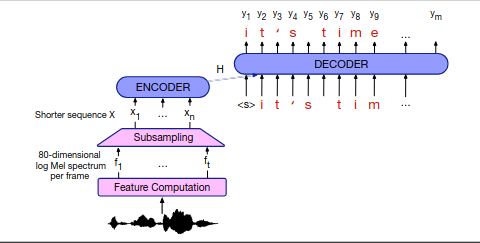
\includegraphics[width=\linewidth]{Latex//sections//images/asrencoderdecoder.png}
    \caption{Schematic architecture for an encoder-decoder speech recognizer from \cite{jm3}}
    \label{fig:asrencoderdecoder schmeatic}
\end{figure}


\subsection{Translation}
Translation is the practice of translating text or language from one language into another language. 
This can be done by hand by a human or in a very statistical approach where a dictionary is used to directly translate the text. 
Another way is with a machine learning approach where a Neural network learns the representations of one language and how this translates in a different language. 
The current standard Machine translation (MT) architecture is an encoder-decoder transformer architecture, which is explained more in depth later. 
As most sentences can be translated independently from each other, this is what is usually done in machine translation. To translate a sentence from the source language into the target language the MT system has to generate the corresponding target sentence. \cite[chapter~13.2]{jm3}

For example the German source sentence: \color{blue}"Der Apfel ist grün." \color{black} would have to be translated into the English sentence \color{blue}"The apple is green"\color{black}. 

For a MT model to be able to do this translation it has to be trained on on data. This data is a large amount of matched sentences in both the source and target languages. The training itself is supervised machine learning; this means the system has to learn how to map the source sentences to the target sentences. To do this the input is encoded into tokens. These can be words, subwords, so parts of words, or characters. It is more useful to do this with units that are smaller than words. These are called subword tokens and they have the advantage that they make it easier to generate the vocabulary of the MT system, which is fixed in advance, usually by the training. 
In an encoder-decoder architecture the encoder will take the input sentence in the source language and produce the context, which is passed to the decoder which produces the decoded target language sentence. \cite[chapter~13.2]{jm3}

%A really common subword tokenization method is Byte Pair Encoding (BPE) \cite[chapter~13.2]{jm3}

\subsection{Speech translation}
Speech translation or spoken language translation is similar to regular translation but it has, like the name says, spoken language as the basis for the translation instead of text.
There are 2 main approaches to Speech Translation (ST): cascaded models, which consist of a ASR model and a MT model, and end-to-end models, which have are only one model, most of the time a encoder-decoder architecture.
Cascaded models have been used for a long time as they are easy to implement. But end-to-end models have gained quite a lot more popularity in the last years as they promise better results and ideas that have proven to work well in text-to-text MT have been tested for ST, with good results.

\subsubsection{Cascaded Models}
Cascaded Speech translation Models consist of 2 parts: a part that is responsible for transcribing the audio, which is usually done with an ASR model, and a part that is responsible for translating the resulting transcription, which is done with neural machine translation or statistical machine translation. A basic overview of this can be seen in \autoref{fig:cascadedmodel}.

\begin{figure}[ht]
    \centering%
    \includegraphics{Latex/sections/images/cascadedmodel.tikz}
\caption{Basic overview of a cascaded speech translation model}
\label{fig:cascadedmodel}
\end{figure}
To train a cascaded ST model one would have to train the ASR system and the MT system. This can be done separately as long as the ASR system is trained for the source language and the MT system is trained to translate form the source to the target language. This makes cascaded systems quite convenient to train as different datasets can be used to train both parts of the model as long as they have vocabulary overlap. 
%TODO citation and expand

\subsubsection{End-to-End Models}
End-to-End Speech translation models do not have the explicit split between the Automatic Speech Recognition model and the translation. This means that such a model gets audio as an input and outputs the text in the target language. 
End-to-End models are trained to perform a task from the raw input, which in the case of Speech translation case is audio, to the output, in this case the corresponding translation, without any intermediate processing from outside the model or feature-engineering in sub-models. This can be seen in \autoref{fig:end-to-end models}. 

\begin{figure}[ht]
    \centering%
    \includegraphics{Latex/sections/images/end-to-end model.tikz}

\caption{basic overview of a end-to-end model architecture}
\label{fig:end-to-end models}
\end{figure}

To train an end to end ST system a dataset with audio and corresponding translations in the target language is needed, as the system has to learn the mapping between the audio sequences and the translated sentences. This process works very similar to the MT training process. However it is significantly more time intensive to create such datasets, especially if a more conversational and casual setting of spoken language is looked for. 


\subsection{Softmax}
Taking the softmax of a vector or probability distribution maps each entry in that probability distribution to a value between 0 and 1 by setting all values below 0 to 0, scaling all values that are bigger than 0 to fall between 0 and 1, as well as making sure that the sum of all the values is 1. 
Mathematically this can be described as $$softmax(z)_i=\frac{exp(z_i)}{\sum_j exp(z_i)}$$ where $z=(z_1\dots z_K)\in R^K$.

So an example of applying the softmax to a probability distribution follows. Let $x= (0, -1, 2, 1, -5, 5)$ be a vector or probability distribution that the softmax is to be applied on. The sum of all non 0 values is $2+1+5=8$. Applying the softmax to each element goes like this: the first element, the 0, stays a 0; the second element, the -1, is negative so the the value is set to 0. The third element, 2, is positive, so it gets scaled down by the sum of all positive values $2/8=0.25$; the fourth element 1 also gets scaled down to 0.125. The fifth element is -5 so it gets set to 0 as well, and the last element in the array is 5 which gets scaled down to be $5/8=0.625$.
This results in the softmaxed vector $softmax(x)=(0,0,0.25,0.125,0,0.625)$. and this fulfills the requirement that $\sum_ix_i = 0+0+0.25+0.125+0+0.625= 1$. \cite[chapter~5.3.1]{jm3}

\subsection{Entropy}
\label{entropy}
In Information theory the entropy is the average amount of uncertainty or information that is found in a discrete probability distribution. More specifically the entropy of a random variable measures the average amount of uncertainty that is connected to that random variable.
The concept of Entropy was proposed by Shannon for the context of measuring the information in transmitted data \cite{shannonentropy}. Entropy is also used in thermodynamics where is is used to denote the randomness, disorder, or uncertainty of systems and it is the central point of the 2. law of thermodynamic.

The entropy is mathematically defined as $- \sum_{x\in \chi} p(x) log p(x)$ ,where p is a probability, $\chi$ is the probability distribution, and $x$ is an element from that probability distribution.


\subsection{Dropout}\label{bg:dropout}
Dropout in the context of machine learning usually refers to the process of dropping out, so omitting, units in the neural network. 
One variation of these dropout methods is Monte-Carlo dropout \cite{gal2016dropoutbayesianapproximationrepresenting}, in short MC dropout, which is the process of masking neurons in a Deep Neural Network randomly, based on a Bayesian probability to 0. A graphic example of this masking values to 0 can be seen in \autoref{fig:dropout}.
This is usually done during training to reduce the chance of the model overfitting on the training data, and this application was first proposed by Srivastava et al. \cite{JMLR:v15:srivastava14a}. 
Nowadays it is very common to use dropout in general and in particular MC dropout during training for this exact reason.

\begin{figure}[ht]
    \centering
    \begin{subfigure}{0.45\textwidth}
        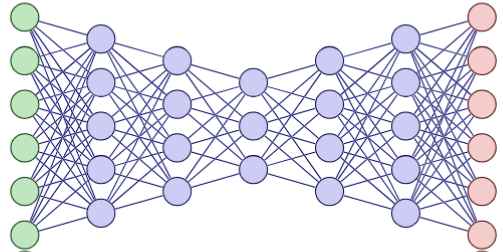
\includegraphics[width=\linewidth]{Latex//sections//images/nondropout.png}
    \end{subfigure}
    \begin{subfigure}{0.45\textwidth}
        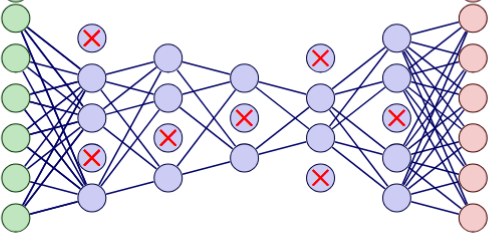
\includegraphics[width=\linewidth]{Latex//sections//images/dropout.png}
    \end{subfigure}
    
    \caption{dropout in a basic Neural Network model}
    \label{fig:dropout}
\end{figure}

Monte Carlo Dropout has also been utilized in Deep Neural Networks to measure the uncertainty of the Network.   
This application of it has been shown in \cite{gal2016dropoutbayesianapproximationrepresenting}. Gal et. al also demonstrate in this that using dropout can be interpreted as a Bayesian approximation of Gaussian processes. To obtain the model uncertainty from this Bayesian approximation they only use the predictive mean and uncertainty of stochastic forward passes. Both the predictive mean and the uncertainty that this delivers are part of the methods used to retrieve quality estimation scores in \autoref{ch:methods} and thus are explained more there.

This use of Monte Carlo dropout is mostly used in deep architectures but is also used to measure the uncertainty in Auto-encoders. \cite{gawlikowski2022surveyuncertaintydeepneural}
The use of dropout to measure the model's uncertainty in Automatic Speech recognition has been tried by Vyas et al. \cite{8683086} before.
They have found that most uncertainty in ASR stems from noisy input data, especially since non-noisy data produces good transcriptions a lot of the time if the model knows all used words and names. 

\section{Models}
\label{ch:models}
All the models used in this thesis use an encoder-decoder architecture, and more specifically transformer architecture models, which is a subsection of encoder-decoder models. Encoder-decoder models are also sometimes called sequence-to-sequence models as they are able to generate sequences of arbitrary length based on the input sequence.
All of the models used are such encoder-decoder models. 

\subsection{Decoder-Encoder}

Encoder-decoder Models are Models that contain an encoder and a decoder. The encoder creates an embedding of the input; this embedding is also called the context or context representation. While embedding the encoder can also add additional context to the representation. 
This context representation is then input into the decoder, which decodes it into a form that is for example a human readable text. 
The basic idea of this can be seen in \autoref{fig:encoderdecodermodel}.
\begin{figure}[ht]
    \centering%
    \includegraphics{Latex/sections/images/encoderdecoder.tikz}
    \caption{basic overview of an encoder-decoder model architecture}
    \label{fig:encoderdecodermodel}
\end{figure}

As mentioned before the encoder-decoder Architecture is used for Sequence-to-Sequence models, since it allows inputting a sequence and outputting a sequence that can be a different length than the input sequence. \cite[chapter~8.7]{jm3}

Using an encoder-decoder architecture as a sequence-to-sequence translation model was first introduced by Sutskever et. al \cite{sutskever2014sequencesequencelearningneural}.
They proposed it using LSTMs, which stands for Long Short Term Memory networks and are a kind of Recurrent neural network (RNN) that can remember information longer than regular RNNs by having a more complex internal structure than RNNs, as the makeup of both the encoder and decoder. 
A simplified example of the translation process that was proposed is pictured in \autoref{fig:encoderdecodertranslationexample}.
\begin{figure}
    \centering
    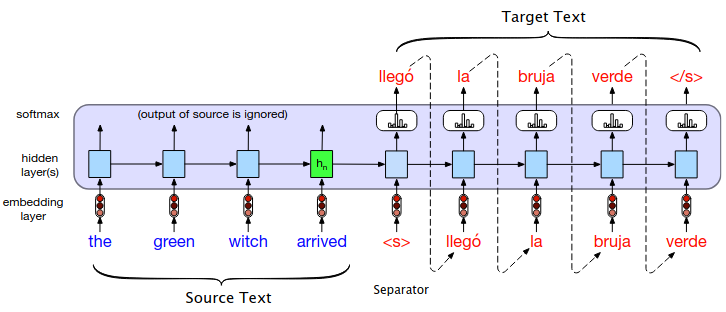
\includegraphics[width=0.5\linewidth]{Latex//sections//images/encoderdecodertranslation.png}
    \caption{Example of a single sentence translation in a basic RNN encoder-decoder approach. The source and target sentence are concatenated with a separator token. The decoder then uses the context information from the last hidden state of the encoder. Taken from \cite{jm3}} 
    \label{fig:encoderdecodertranslationexample}
\end{figure}


\subsection{Transformer}
The Transformer architecture is a Neural Network architecture that was first introduced in the paper Attention is all you need \cite{vaswani2023attentionneed} that makes use of self-attention mechanisms. 

The attention mechanism is responsible for weighing and combining the representations from other relevant tokens in the context of the layer k-1 to create the representation for tokens in layer k. This creates contextual embeddings for words in a sequence by adding meaning from contextually relevant words to the embedding. 
Self-attention mechanisms make use of this attention and also use information from all previous representations in the context window. Depending on the model the transformer's self-attention mechanism can also make use of the representations of later tokens. This all describes a single attention head; the transformer has several of these which attend to different purposes in the context.

The Transformer has an encoder-decoder structure with N encoder blocks that are made up out of Multi-Head Attention blocks and feed forward networks. Both of these have an add and normalization layer behind that, which each take the input token $x_i$, where i is the position of the token, put it through the Multi-Head Attention add it back to $x_i$. This is then put into the feed forward network and added back onto the previous result. This process can be seen in \autoref{fig:transformermodel} along with the general architecture of the transformer. 
The N blocks can map an entire context window of input vectors $(x_1\dots x_n)$ to a of the same length window of output vectors $(h_1\dots h_n)$. 
The decoder part consists of N blocks that contain a Masked multi-head attention block, a Multi-layer attention block, and a feed forward neural network. In the end there is a linear layer and a softmax layer. \cite[chapter~9]{jm3}

\begin{figure}[ht]
        \centering%
        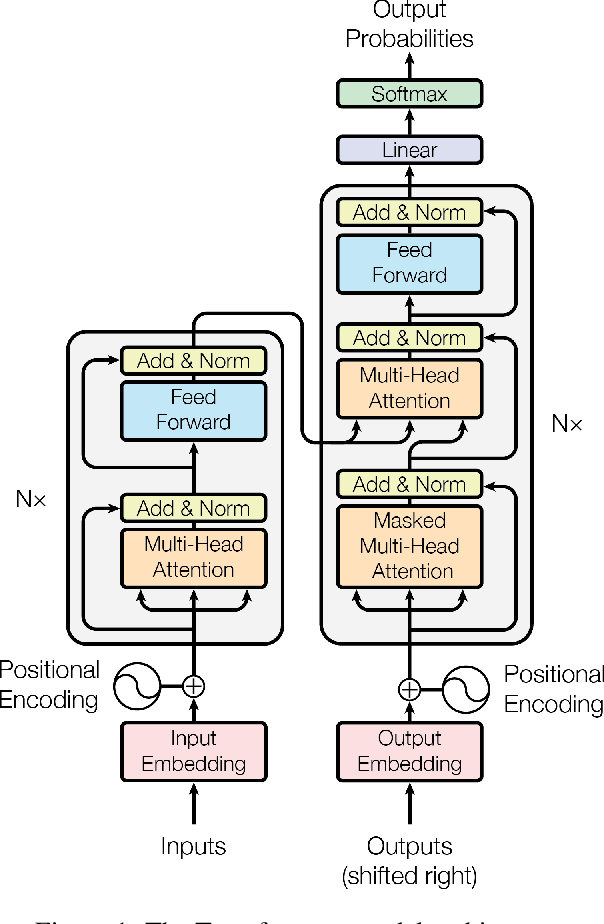
\includegraphics[width=0.5\linewidth]{Latex//sections//images/transformermodel.png}
        \caption{Transformer model architecture Vaswani et. al 2017}
        \label{fig:transformermodel}
    \end{figure}


\subsection{Whisper}
Whisper is a multilingual multitask Model that is focused on speech processing and was proposed in the Robust Speech Recognition via Large-Scale Weak Supervision paper \cite{radford2022robust}. 
Its architecture is based on a classical Transformer Architecture where the Transformer encoder Blocks consist of self attention blocks and Multilayer perception blocks. 
The Transformer decoder blocks use the learned position embeddings and tied input-output token representations. 
The encoder and decoder have the same number of transformer blocks.
The audio pre-processing is done by making sure the audio chunks that are given to the model are 30 seconds long, have ben sampled to 16,000 Hz, and have a 80-channel log-magnitude Mel spectrogram representation. This log-mel spectrogram is then computed with 25-millisecond windows and a stride of 10 milliseconds. If an audio chunk is shorter than 30 seconds it gets padded up to 30 seconds; if it is longer the audio gets split up. 
This input is then scaled to be between -1 and 1 and is put through 2 convolutional layers that have a filter width of 3 and use the GELU function as activation function. The second of those 2 layers has a stride of 2. 
The resulting data is then added to a sinusoidal position embedding, which is a positional encoding embedding that uses sinusoidal functions, so the sine and cosine \cite{vaswani2023attentionneed}, and then forwarded into the encoder blocks.

\begin{figure}
        \centering%
        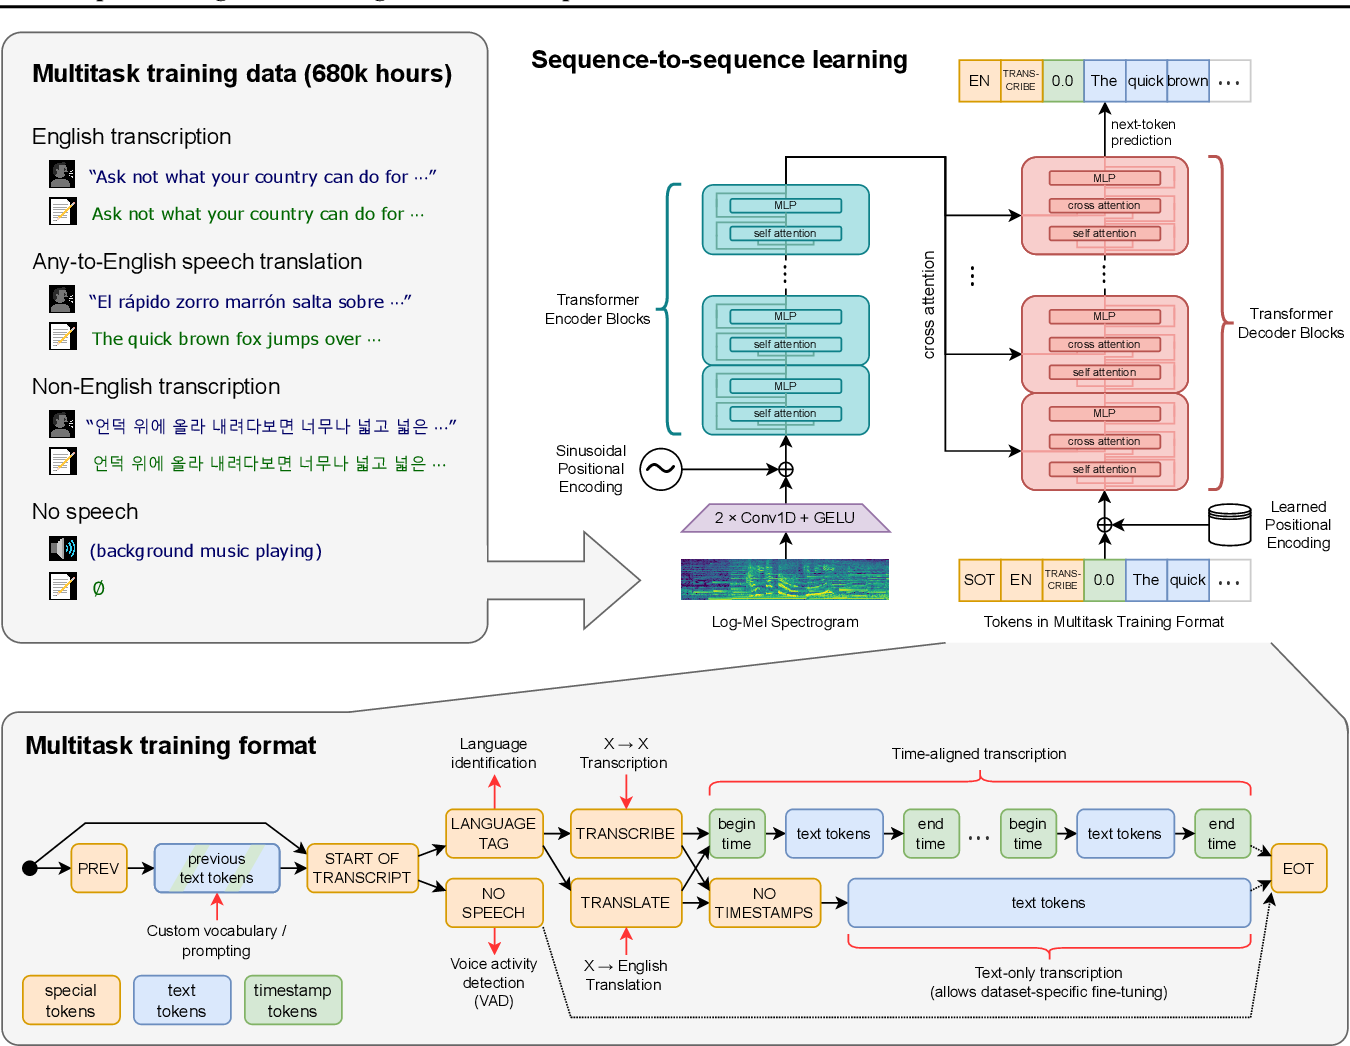
\includegraphics[width=0.5\linewidth]{Latex//sections//images/whispermodel.png}
        \caption{Overview of the Whisper architecture Radford et. al 2022}
        \label{fig:whispermodel}
    \end{figure}



\subsection{Seamless}
Seamless \cite{seamless2023} is a multilingual, multimodal model that uses a transformer architecture for the text translation part and, in the v2 version which is used in the experiments, it uses a w2v-Bert speech encoder which was pretrained on unlabelled audio data. 
The general architecture of Seamless is shown in \autoref{fig:seamlessmodel}, for this thesis only the left half up to the Transformer Text decoder of the figure is relevant, the other parts of it are used for speech synthesis.

\begin{figure}
        \centering%
        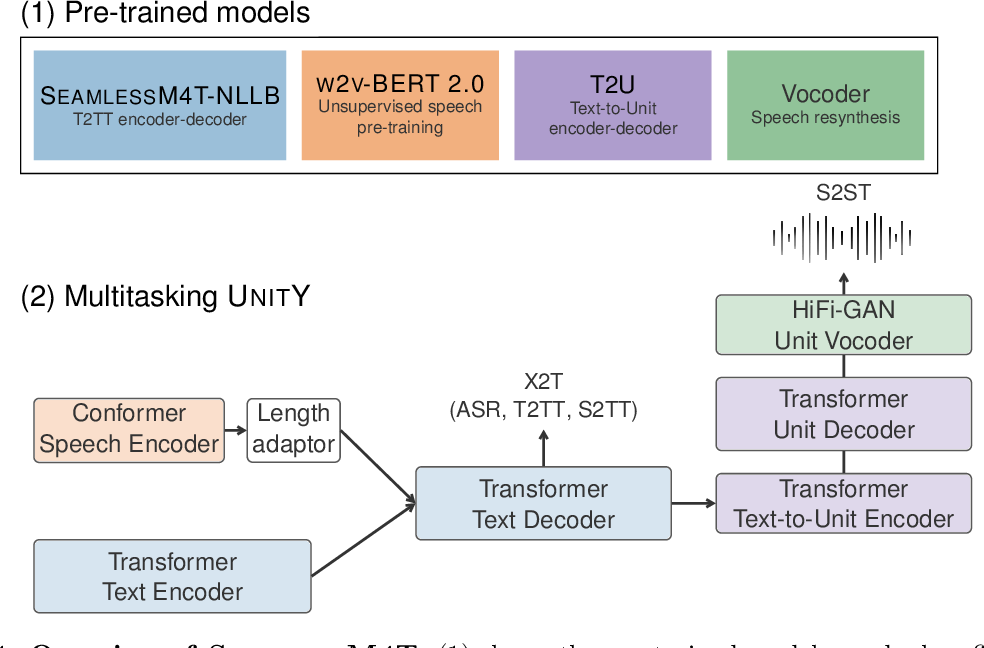
\includegraphics[width=0.7\linewidth]{Latex//sections/images/seamlessmodel.png}
        \caption{Overview of SeamlessM4T. (1) shows the pre-trained models used when finetuning multitasking UnitY. (2) outlines multitasking UnitY with its two encoders, text decoder, T2U encoder-decoder, and the supporting vocoders for synthesizing output speech in S2ST. \cite{seamless2023}(figure 4)}
        \label{fig:seamlessmodel}
\end{figure}

Seamless v2 improves upon the original model by introducing non-autoregressive text-to-unit decoding. However, this modification has minimal impact on this thesis since it primarily focuses on text-to-text (T2TT) and speech-to-text (S2TT) translation. 
The other change for v2 is that it uses a w2v-Bert 2.0 \cite{chung2021w2vbertcombiningcontrastivelearning} encoder that is trained self-supervised on 4.5 million hours of unlabled audio, as compared to the previous 1 million hours of unlabeled data.
SeamlessM4T has been trained on unlabeled, human-labeled, pseudo-labled, and automatically aligned data, where the text-to-text-translation (T2TT) was done on NLLB data \cite{nllbteam2022languageleftbehindscaling}. This is a method of creating low-resource language datasets with a combination of using the Flores \cite{guzmán2019floresevaluationdatasetslowresource} and No Language Left Behind (NLLB) Seed dataset, which is a set of professionally translated sentences in the Wikipedia domain. 
% from seamless v2 paper
The anything-to-text model, which can do T2TT, ASR, and Speech to Text translation (S2TT), is trained on different sources of S2TT data that is human-labeled, pseudo-labeled, and automatically aligned, and is a combines the v2w-Bert model and the Text encoder from the NLLB T2TT model and the corresponding decoder.
It was trained in 2 steps on this data; the first one focuses on supervised English ASR and S2TT data where the target language is English. 
The 2. step in training then focuses on English to X S2TT and non-English ASR data.

The experiments were run on the v2 large version, both for the cascaded part and the end-to-end part of the experiments, no additional training was used.

%TODO read further
\subsection{SentencePiece}
SentencePiece \cite{kudo-richardson-2018-sentencepiece} is a tokenizer and detokenizer that allows for subword units, especially byte pair-encoding \cite{sennrich-etal-2016-neural}, that are language independent, as the sentences are treated as unicode character sequences and preprocessing is not always needed. 
It's comprised of a Normalizer, a Trainer, an encoder, and a decoder. 
The encoder uses the Normalizer to normalize the Test and then tokenizes the sentence. 
In the SentencePiece implementation the Decoding is considered the inverse operation of Encoding of normalized text. This results in a lossless tokenization, so there is no information loss over the process of encoding and decoding. 
To achieve this SentencePiece encodes white spaces with a meta-symbol that can be reverted. 
SentencePiece also manages the Vocabulary that is used in preprocessing as it also outputs a dictionary and can output a ID sequence to text and vice versa mapping. 
As the SentencePiece model is self-contained it also leads to better reproducibility as only the model file is needed, which is publicly available. 

\subsection{DeltaLM}
DeltaLM \cite{ma2021deltalm} is one of the current state of the art Neural Machine Translation models. 
It is based off of the classical encoder-decoder structure but both the encoder and decoder are initialised with the pretrained multilingual encoder and then trained in a self-supervised manner. In classical pretrained encoder-decoder architectures only the encoder is initialized with a pretrained encoder and the decoder is initialized with random values.

In addition to this is the decoder a Interleaved Transformer decoder, which is not the same architecture as the encoder and differs from the standard Transformer decoder in that the Transformer blocks now consist of a self-attention layer, two feed-forward networks, and a cross-attention layer which are arranged as seen in \autoref{fig:interleaved decoder}. 
This way of building the decoder is more similar to the structure of the encoder and makes it easier to leverage the pretrained encoder. 

The interleaved decoder is then initialised with the layers from the pretrained encoder, which is the InfoXLM \cite{chi2021infoxlminformationtheoreticframeworkcrosslingual}, in the following way: the self-attention and the bottom FFN layers are initialised with the odd layers of the InfoXLM encoder and the cross-attention and top FFN layers are initialised with the even layers. 
The leftover components of the decoder are also initialised the same as the pretrained encoder. 
This means that all of the sublayers are initialised with the pretrained weights and none of them use randomised values. 

\begin{figure}
    \centering%
    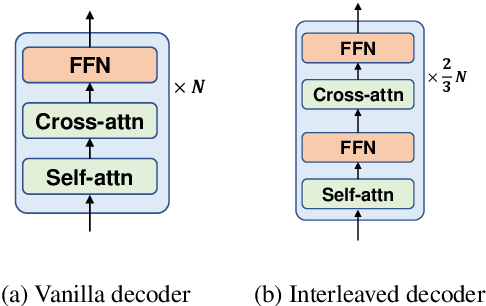
\includegraphics[width=0.5\linewidth]{Latex/sections/images/interleaveddecoder.png}
    \caption{Vanilla Transformer decoder (left) compared to the interleaved Transformer decoder(right) from Ma et. al 2021}
    \label{fig:interleaved decoder}
    %source dlm paper
\end{figure}



\section{Evaluation metrics}
 For the evaluation of the results a couple of terms, algorithms, and methods are used. The explanation of them is in this section. 
 
\subsection{WER}
\label{wer}
The Word Error Rate, in short WER, has been proposed in \cite{woodard1982} and \cite{morris2004}.
It's based on the Levenshtein distance \cite{Levenshtein1965BinaryCC} but instead of working on phonemes it operates on words.
The WER can be computed as $$WER=\frac{S+D+I}{N}=\frac{S+D+I}{S+D+C}$$ where $S$ is the number of substitutions, $D$ is the number of deletions, $I$ is the number of insertions, $N$ is the number of words in the reference, and $C$ is the number of correct words.

\subsection{Comet}
Comet, in full Cross-lingual Optimized Metric for Evaluation of Translation, is a neural framework for machine translation evaluation that was proposed in \cite{rei-etal-2020-comet} and improved in \cite{rei-etal-2022-comet}.
For this thesis the Estimator model is relevant, which is used to estimate a quality score based off of a source sentence and a translation reference. The estimator model architecture is pictured in \autoref{comet architecture}.

To do this the hypothesis translation, the source sentence, and the reference translation are encoded independently using a pre-trained encoder, that is a cross-lingual model like XLM \cite{lample2019crosslinguallanguagemodelpretraining}, a multilingual BERT \cite{devlin2019bertpretrainingdeepbidirectional}, or XLM-RoBERTa \cite{conneau2020unsupervisedcrosslingualrepresentationlearning}. The resulting embeddings are padded into a pooling layer where they create a sentence embedding for each segment. The Embeddings are then combined and concatenated into a single vector that is passed into a regression layer, that then regresses on reference scores from Direct Assesment (DA) \cite{graham-etal-2013-continuous}, MQM \cite{mqm}, and HTER \cite{snover-etal-2006-study}.
This model is trained to minimize the Mean Squared error. 

In the original implementation this does not give a score from 0 to 1 based on how good or bad the translation is, but the improved version does this, where a score of 1 means a perfect translation and a score of 0 means a bad translation. Besides this, only hyper-parameters have been changed in comparison to the original version, and more training has been done.
\begin{figure}[ht]
    \centering
    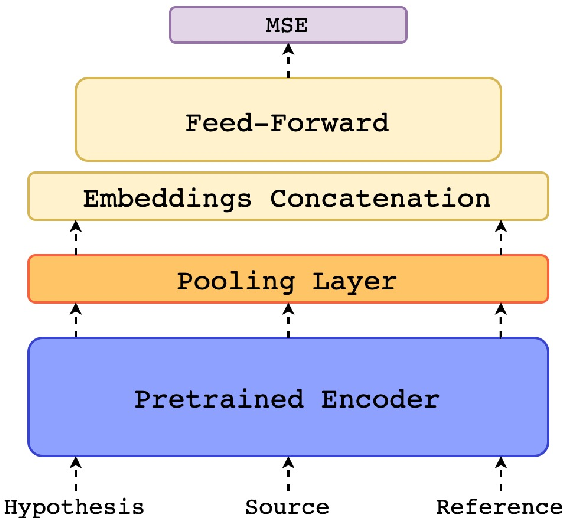
\includegraphics[width=0.3\linewidth]{Latex//sections//images/cometestimatormodel.png}
    \caption{overview of the comet estimator model architecture from \cite{rei-etal-2020-comet}}
    \label{comet architecture}
\end{figure}


\subsection{Pearson-correlation}
The Pearson correlation, or Pearson correlation coefficient (PCC), is a method to see how correlated 2 sets of values are. The r value is the covariance of the 2 sets divided by the product of their standard deviations $$PCC(x,y) =\frac{\sum_{i=1}^n (x_i-\overline{x})(y_i-\overline{y})}{\sqrt{\sum_{i=1}^n (x_i-\overline{x})^2}\sqrt{\sum_{i=1}^n(y_i-\overline{y}})^2}$$ where $\overline{x},  \overline{y}$ are the means of the sets of values, $x_i, y_i$ are individual elements of the set of values, and $n$ is the sample size. 
Due to this definition the possible values for the PCC are between -1 and 1, where a value of 1 means the sets are correlated, so a linear relation between the 2 value sets exists. A value of -1 is the result of the PCC if it's inversely correlated. 
If the value is 0 calculated this means the sets are not correlated at all. A graphical representation of these scores can be found in \autoref{fig:pearosncorr}. \cite{pearsoncorr}
\begin{figure}[ht]
    \centering
    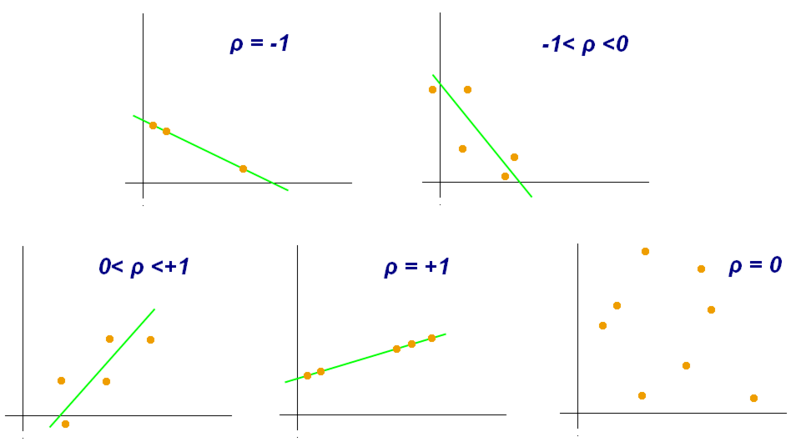
\includegraphics[width=0.7\linewidth]{Latex//sections//images/pearson correlation.png}
    \caption{graphical representation of different Pearson correlation scores \cite{pearsoncorrimage}}
    
    \label{fig:pearosncorr}
\end{figure}

The PCC has the advantage that it's symmetric, so switching the order of the inputs does not change the correlation score, but it has the drawback that it can be numerically unstable.% This means that if the values in the sets are right the Pearson correlation the most significant digits are eliminated and digits that are prone to rounding errors are the new most significant digits. 
